\section{Interaction Methods in 3d Environment}
There are different ways of conveying a 3D environment within the smart device spectrum, in this case smartphones and tablets. It is important that the aim of the project is established before moving on to conclusions on which approach to take. Since the project revolves around navigation in a three dimensional environment, irrelevant approaches will be eliminated right away.

A very important part when developing the application to fit a great\todo{Originally said pleasurable, might need revising} user experience is to make sure that it works as flawless as possible and that there are no misinterpretations when using the product. For the product that is going to be developed, the "traditional" interaction methods do not cover the functionalities that are needed to cover our initial concept needs. To assure that the alternative interaction is integrated in a convenient manner, knowledge about different sensors and possible combination of two or more to make more intelligent outcomes should be established.

%It is also important to note that the proportions will differ from reality because of the devices' size. This project is aimed at visual representation of a rather realistic environment and will be taken into account during the implementation. \todo{also not sure if this part is necessary here}

\subsection{Traditional interaction}
As technology evolves, new ways of interacting with computational devices are constantly built. With that, people's needs also change. People adapt to new ways of communication with technology. \cite{Greenfield}
The transition from the classical buttons on a cellphone to a touchscreen has made new ways of interaction possible - the delimitation of physical buttons made it available to have any customized graphical interfaces on the screen possible. This made life easier for casual tasks like zooming a photo using two fingers as multi touch input. This allows registration of multiple points of contact simultaneously, which is much more intuitive than the classical button alternative.
Soon enough non-traditional sensors started finding their place in smartphones. The implementation of these sensors in the smartphone allowed new forms of interaction, such as video calling, flashlight and screen orientation, followed by more interesting unusual uses. Application developers started making instrument tuners (GStrings), barcode scanners (Barcode Scanner), radiation detectors (GammaPix), pulse detectors (Instant Heart Rate), light intensity meters (Light Meter) and countless other applications that uses the sensors to their favour in a non-traditional manner. However, we will only focus on sensors that support our problem area, which points to the ones that can work with 3D environments. The relevant ones for this project are the gyroscope, accelerometer and magnetometer.

\subsection{Sensors} \label{sensors}

As it has been established so far there are three main sensors that can support orientation in 3D environments possible. These sensors are accelerometer, gyroscope and magnetometer. In the following section it will be determined whether these sensors are in fact useful to this project's case and if so, to what extent.

\subsubsection*{Gyroscope, Accelerometer and Magnetometer}
Gyroscope, Accelerometer and Magnetometer are the three sensors that most of the newer smartphones have \cite{AndroidDevelopers} that can measure orientations on X, Y and Z axis, allowing the apps to calculate placement of the device in the 3D environment.

Gyroscope can be used to help determine orientation using gravity.\todo{REFERENCES} Since it detects rotation in three dimensional space, it can be used in favour of this project to convey the rotation that is in a way similar to the one that is natural i.e. in eyesight. Gyroscope, in comparison to magnetometer and accelerometer, is the physically largest and most expensive sensor, so the possible limitations in the smart devices in-built Gyroscopes have to be considered.

\begin{figure}[H]
\centering
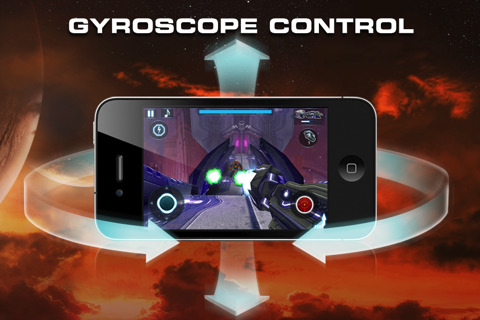
\includegraphics[scale=0.5]{GyroscopeApp.jpg}
\caption{iPhone game using a gyroscope sensor}
\end{figure}

The accelerometer can support other sensors to give the impression of the environment representation in three dimensional space. This helps to stabilize the view angle to represent real world by giving the position perpendicular to the Earth's surface. In other words, it would eliminate wrong position starting point - moving forward horizontally in reality while in the virtual environment it goes upside down could cause cluster. Accelerometer, along with other sensors is commonly used in the augmented reality concepts (Yelp Monocle, Google Ingress, SpecTrek etc). The world position calculation is not necessary for an app that is being developed, but it could be useful when wanting to change between landscape and portrait modes, if the need is established in further design iterations.

The last sensor that is able to collect three dimensional data is the magnetometer. It is typically used to measure the absolute position of the three dimensional orientation in terms of Geographical placement on earth, which is irrelevant for this project. Additionally, magnetic interference can disturb its flow, which may lead to inaccurate results. In future development of the project, an online feature with more precise positioning in relation to other users could be considered. Alternatively, the magnetometer can be used to support the gyroscope and accelerometer with positioning, if they lack precision axis-wise. If there are no problems with accelerometer and gyroscope axis measurement i.e. blind spots that these two sensors can not recognize - implementation of the magnetometer is not necessary. 

\begin{figure}[H]
\centering
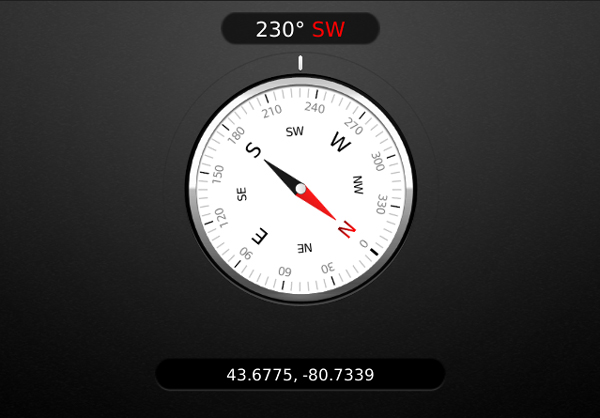
\includegraphics[scale=0.5]{MagnetometerApp.jpg}
\caption{a simple compass app that establishes the magnetometer sensor}
\end{figure}

\begin{figure}[H]
\begin{subfigure}{.5\textwidth}
  \centering
  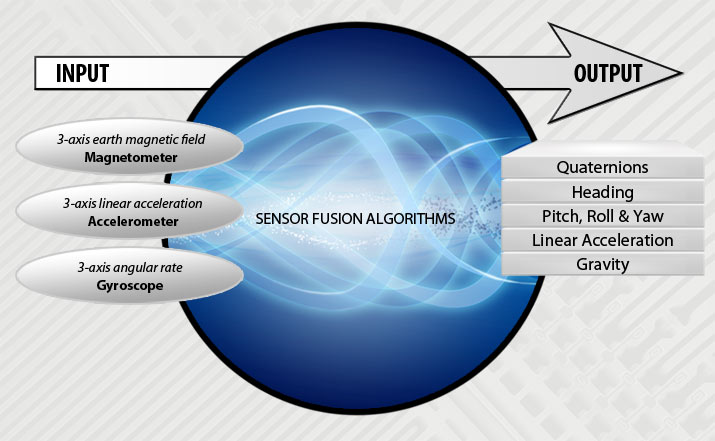
\includegraphics[width=.9\linewidth]{Sensors.jpg}
\end{subfigure}%
\begin{subfigure}{.5\textwidth}
  \centering
  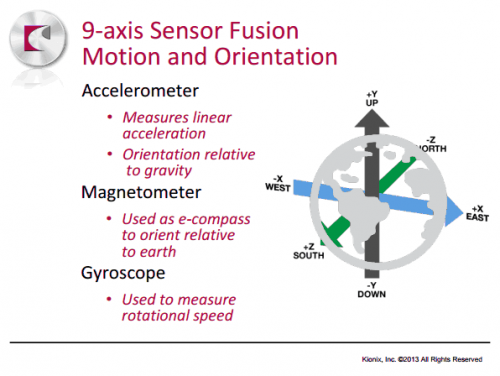
\includegraphics[width=.9\linewidth]{Sensors2.png}
\end{subfigure}
\caption{uses of sensors}
\end{figure}


\subsection{Conclusion}
The sensors discussed in earlier sections will help us work towards establishing that the perception of 3D environments is ensured to be conveyed in the best manner. After gaining more knowledge it can be seen that there is a variety of options how the use of sensors can be enabled in different application contexts.